\section{Background}\label{sec:background}

\subsection{GraphBLAS}

Basic ideas. 

Problems (implicit zeroes, etc).

SuiteSparse:GraphBLAS as a reference implementation

LAGraph as a collection of graph analysis algorithms (based on SuiteSparse:GraphBLAS). 

\subsection{Tree-based Representation for Sparse Matrices and Vectors}

To store sparse matrices and vectors efficiently, we employ a quad-tree data structure. The matrix is recursively subdivided into four quadrants~--- northwest (NW), northeast (NE), southwest (SW), and southeast (SE)~--- until each block becomes either uniform or empty.
The figure~\ref{fig:quadtree_example} shows an example of a matrix in the quad-tree form.

\begin{figure}[htbp]
    \centering
    \caption{Example of the matrix and its quad-tree representation}
\begin{subfigure}[b]{0.9\textwidth}
    \centering
    \caption{Block decomposition of the matrix}
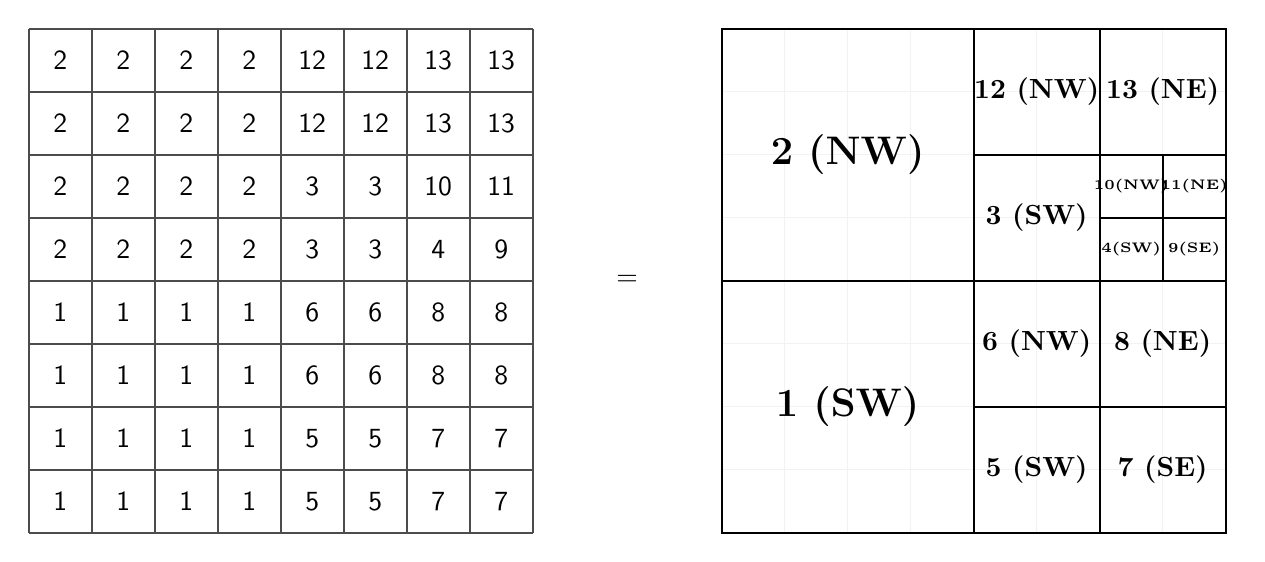
\begin{tikzpicture}[scale=0.8, font=\sffamily]

  \draw[step=1cm, black!70, thick] (0,0) grid (8,8);
  
  \foreach \x/\y/\val in {
    0/0/1, 1/0/1, 2/0/1, 3/0/1, 4/0/5, 5/0/5, 6/0/7, 7/0/7,
    0/1/1, 1/1/1, 2/1/1, 3/1/1, 4/1/5, 5/1/5, 6/1/7, 7/1/7,
    0/2/1, 1/2/1, 2/2/1, 3/2/1, 4/2/6, 5/2/6, 6/2/8, 7/2/8,
    0/3/1, 1/3/1, 2/3/1, 3/3/1, 4/3/6, 5/3/6, 6/3/8, 7/3/8,
    0/4/2, 1/4/2, 2/4/2, 3/4/2, 4/4/3, 5/4/3, 6/4/4, 7/4/9,
    0/5/2, 1/5/2, 2/5/2, 3/5/2, 4/5/3, 5/5/3, 6/5/10, 7/5/11,
    0/6/2, 1/6/2, 2/6/2, 3/6/2, 4/6/12, 5/6/12, 6/6/13, 7/6/13,
    0/7/2, 1/7/2, 2/7/2, 3/7/2, 4/7/12, 5/7/12, 6/7/13, 7/7/13
  } {
    \node at (\x+0.5, \y+0.5) {\val};
  }

\node at (9.5, 4) {$=$};

\begin{scope}[shift={(11,0)}]
    \draw[step=1cm, gray!10, very thin] (0,0) grid (8,8);
    
    \draw[draw=black, thick] (0,4) rectangle ++(4,4) node[midway, font=\Large\bfseries] {2 (NW)};
    \draw[draw=black, thick] (0,0) rectangle ++(4,4) node[midway, font=\Large\bfseries] {1 (SW)};
    
    \draw[draw=black, thick] (4,6) rectangle ++(2,2) node[midway, font=\bfseries] {12 (NW)};
    \draw[draw=black, thick] (6,6) rectangle ++(2,2) node[midway, font=\bfseries] {13 (NE)};
    \draw[draw=black, thick] (4,4) rectangle ++(2,2) node[midway, font=\bfseries] {3 (SW)};
    
    \draw[draw=black, thick] (6,4) rectangle ++(1,1) node[midway, font=\tiny\bfseries] {4(SW)};
    \draw[draw=black, thick] (7,4) rectangle ++(1,1) node[midway, font=\tiny\bfseries] {9(SE)};
    \draw[draw=black, thick] (6,5) rectangle ++(1,1) node[midway, font=\tiny\bfseries] {10(NW)};
    \draw[draw=black, thick] (7,5) rectangle ++(1,1) node[midway, font=\tiny\bfseries] {11(NE)};
    
    \draw[draw=black, thick] (4,2) rectangle ++(2,2) node[midway, font=\bfseries] {6 (NW)};
    \draw[draw=black, thick] (6,2) rectangle ++(2,2) node[midway, font=\bfseries] {8 (NE)};
    \draw[draw=black, thick] (4,0) rectangle ++(2,2) node[midway, font=\bfseries] {5 (SW)};
    \draw[draw=black, thick] (6,0) rectangle ++(2,2) node[midway, font=\bfseries] {7 (SE)};
    

  \end{scope}
\end{tikzpicture}

\label{fig:quadtree_blocks}
\end{subfigure}

\vspace{1cm}

\begin{subfigure}[b]{0.9\textwidth}
    \centering
    \caption{Quadtree representation of the blocks in~\ref{fig:quadtree_blocks}}
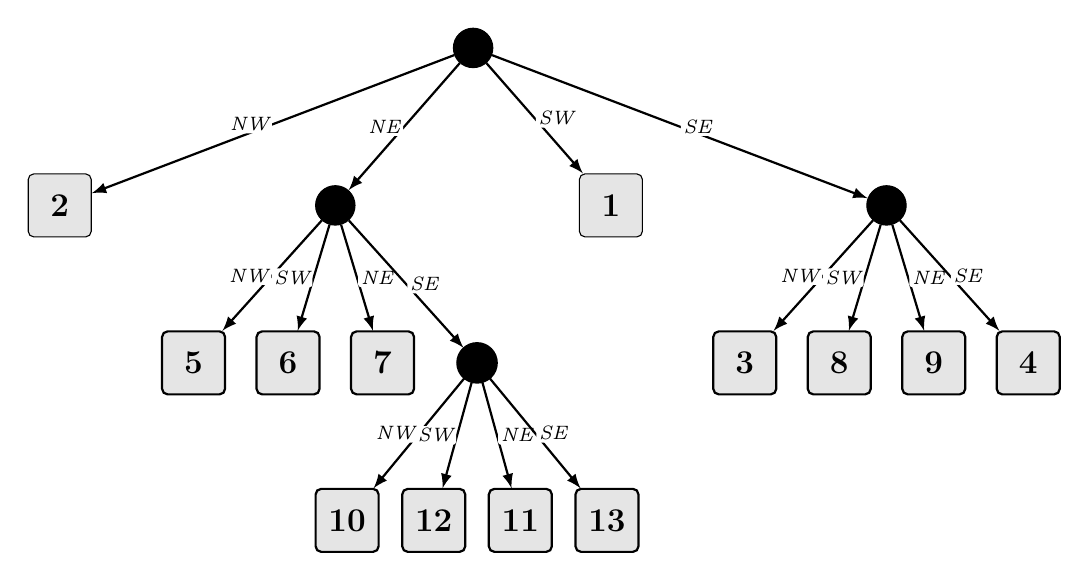
\begin{tikzpicture}[
    grow=down,
    level 1/.style={sibling distance=3.5cm, level distance=2cm},
    level 2/.style={sibling distance=1.2cm, level distance=2cm},
    level 3/.style={sibling distance=1.1cm, level distance=2cm},
    edge from parent/.style={draw, -latex, thick},
    int/.style={draw, circle, fill=black, font=\small\bfseries, minimum size=0.5cm, inner sep=0pt},
    leaf/.style={draw, rectangle, fill=gray!20, font=\large\bfseries, minimum size=0.8cm, inner sep=2pt, rounded corners=2pt},
    q/.style={font=\scriptsize\itshape, pos=0.5, fill=white, inner sep=1pt, rounded corners=1pt}
]

\node[int] { }
    child { node[leaf] {2} edge from parent node[q, left] {NW} }
    child {
        node[int] { }
        child { node[leaf] {5} edge from parent node[q, left] {NW} }
        child { node[leaf] {6} edge from parent node[q, left] {SW} }
        child { node[leaf] {7} edge from parent node[q, right] {NE} }
        child {
            node[int] {}
            child { node[leaf] {10} edge from parent node[q, left] {NW} }
            child { node[leaf] {12} edge from parent node[q, left] {SW} }
            child { node[leaf] {11} edge from parent node[q, right] {NE} }
            child { node[leaf] {13} edge from parent node[q, right] {SE} }
            edge from parent node[q, right] {SE}
            }
        edge from parent node[q, left] {NE}
    }
    child { node[leaf] {1} edge from parent node[q, right] {SW} }
    child {
        node[int] { }
        child { node[leaf] {3} edge from parent node[q, left] {NW} }
        child { node[leaf] {8} edge from parent node[q, left] {SW} }
        child { node[leaf] {9} edge from parent node[q, right] {NE} }
        child { node[leaf] {4} edge from parent node[q, right] {SE} }
        edge from parent node[q, right] {SE}
    };
\end{tikzpicture}
\label{fig:quadtree_tree}
\end{subfigure}
\label{fig:quadtree_example}
\end{figure}



This recursive partitioning allows large uniform blocks to be represented implicitly, eliminating the need to store them explicitly.
Unlike flat array formats such as CSR or CSC, which are standard in libraries like SuiteSparse:GraphBLAS, the quad-tree naturally supports a divide-and-conquer execution model and adapts dynamically to irregular sparsity patterns.
This structure simplifies parallelization, as independent sub-blocks can be processed recursively without global synchronization.

However, this flexibility comes at a cost: for dense or highly regular matrices, the overhead of maintaining tree metadata and pointer indirection can outweigh the benefits of sparse storage, making traditional linear formats more efficient in such cases.


\subsection{Interaction Nets}

\label{sec:interaction_nets}

We utilize the variant of definitions provided by Y. Lafont in 1989~\cite{10.1145/96709.96718}. Interaction Nets is a graph-rewriting model where computation proceeds through local rewriting rules applied to pairs of connected nodes.

\textit{(Agent)}. An \textit{agent} is a symbol from a fixed alphabet $\Sigma$, for which:
\begin{itemize}
    \item an arity is defined --- a function $Ar: \Sigma \to \mathbb{N} \cup \{0\}$;
    \item there is one \textit{principal port} and a number of \textit{auxiliary ports} equal to its arity.
\end{itemize}

\textit{(Net)}. A \textit{net} over the alphabet $\Sigma$ is a labeled undirected multi-graph in which:
\begin{itemize}
    \item each node is labeled by an agent;
    \item edges can only exist between ports;
    \item at most one edge enters each port.
\end{itemize}

Let $\mathcal{N}_\Sigma$ denote the set of all possible nets over the alphabet $\Sigma$.

We say that a port is \textit{free} if no edge originates from it. A net can also consist simply of a set of edges, in which case each end of an edge is considered a free port.

\textit{(Interface)}. The \textit{interface} $I(n)$ is the set of all free ports of a net $n$.

We say that port $p_a$ is connected to port $p_b$ if there is an edge between them.
An example of a simple net is shown in figure~\ref{fig:in_example}.
The set of agents is $\Sigma=\{\beta, \alpha\}$ with arities $Ar(\beta)=0$, $Ar(\alpha)=2$.
The principal ports of the $\alpha$-nodes are connected to each other, and the principal port of the $\beta$-node is connected to one of the auxiliary ports of the left $\alpha$-node.
There are three free ports: one at the left $\alpha$-agent and two at the right $\alpha$-agent.
These constitute the interface.

\begin{figure}[h]
    \centering
    \caption{Example of a net consisting of three nodes}
    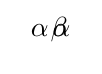
\begin{tikzpicture}
        \matrix[column sep = 1em]{
            \inetcell(b) {$\phantom x\alpha\phantom x$}[R] &
            \inetcell(a) {$\phantom x\alpha\phantom x$}[L]   \\
        };
        \inetcell[left = of b.left pax, distance=1em](out) {$\beta$}[R]
        \inetwirefree(a.left pax)
        \inetwirefree(a.right pax)
        \inetwire(a.pal)(b.pal)
        \inetwire(b.left pax)(out.pal)
        \inetwirefree(b.right pax)
    \end{tikzpicture}
    \label{fig:in_example}
\end{figure}


Computation in Interaction Nets occurs via \textit{reductions}: rewriting an \textit{active pair} into a net. An active pair is defined as two agents connected via their principal ports.

\textit{(Reduction Rule)}. A \textit{reduction rule} is a graph rewriting rule. Let $R$ be the set of reduction rules. More formally, a reduction rule is a triplet $r \in \Sigma \times \Sigma \times \mathcal{N}_\Sigma$, for which the following properties hold:
\begin{itemize}
    \item \textbf{Symmetry:} $(l_1, l_2, n) \in R \Rightarrow (l_2, l_1, n) \in R$
    \item \textbf{Determinism:} $(l_1, l_2, n_1) \in R \land (m_1, m_2, n_2) \in R \Rightarrow (l_1, l_2) \neq (m_1, m_2)$
    \item \textbf{Interface Preservation:} $\forall (l_1, l_2, n) \in R, Ar(l_1) + Ar(l_2) = \|I(n)\|$
\end{itemize}


As shown in Lafont's work~\cite{10.1145/96709.96718}, $\lambda$-calculus can be expressed through this formalism. Additionally, reductions can be performed independently of each other and it has been proven that the order of reductions doesn't matter. This serves as the primary reason for the natural suitability of Interaction Nets for parallel computations.

\subsection{Inpla}

Introduce Inpla: runtime (VM) and language.
Briefly describe its syntax for defining agents and rules, and how it allows to program these graph-rewriting systems.
This section sets the stage for understanding our Inpla-based implementation.

\subsection{Vine}

IVY, IVM. Differences with Inpla.